\section{Introduction}


In the last few decades, quantum computing has become a very active field of research. The main reason for this is the fact that quantum computers promise to outperform classical computers in certain tasks. The most famous example of this is Shor's algorithm \cite{shor1994algorithms} which can factorize large numbers in polynomial time. This is a problem that is believed to be intractable for classical computers. Another example is Grover's algorithm \cite{grover1996fast} which can search an unsorted database in $\mathcal{O}(\sqrt{N})$ time. This is a quadratic speedup compared to the classical $\mathcal{O}(N)$ time.

Usually those algorithms described in a very high-level "language", the so called (quantum-) circuit model. This allows for a very intuitive way reasoning about quantum algorithms, because every unitary operation applied to the quantum state can be compactly represented by a single gate. However, this model does not take the restrictions of real quantum computers into account. \cite{equivalence_checking_tum}

\subsection{Quantum Circuit Compilation}

Real quantum computers come with a set of restrictions. For example, the set of gates is typically limited to a small set of universal gates (e.g. the Clifford+T gate set). Furthermore, the connectivity of the qubits is limited. This means that not every operation can be applied to every pair of qubits. As a consequence, the original circuits needs to be \textit{compiled} into a circuit that can be executed on the specific quantum computer. This process is called \textit{quantum circuit compilation}.



\begin{figure}[h!]
    \centering
    \begin{quantikz}
        \lstick{$\ket{c_1}$} & \ctrl{1}  & \qw\\
        \lstick{$\ket{c_2}$} & \ctrl{1} & \qw \\
        \lstick{$\ket{t}$}   & \targ{}  & \qw
    \end{quantikz}
    \caption{The Toffoli gate.}
    \label{fig:toffoli_gate}
\end{figure}

\begin{figure}[h!]
    \centering
    \begin{quantikz}[row sep=0.3cm, column sep=0.2cm]
        \lstick{$\ket{a}$} & \qw& \qw &\qw & \ctrl{2}& \qw & \qw & \qw & \ctrl{2} & \ctrl{1} & \gate{T} & \ctrl{1} & \qw \\
        \lstick{$\ket{b}$} & \qw&  \ctrl{1}  & \qw  & \qw & \qw & \ctrl{1} & \gate{T} & \qw  & \targ{} & \gate{T^\dagger} & \targ{} & \qw \\
        \lstick{$\ket{c}$} &\gate{H}& \targ{}  & \gate{T^\dagger} & \targ{} & \gate{T} & \targ{} & \gate{T^\dagger} & \targ{} & \gate{T} & \gate{H} & \qw & \qw\\
    \end{quantikz}
    \caption{Decomposition of the Toffoli gate in the Clifford+T gate set.}
    \label{fig:toffoli_decomposition}
\end{figure}



In circuit \ref{fig:toffoli_gate} the Toffoli gate is shown. However it is not represented in the Clifford+T gate set. In order to execute this circuit on a real quantum computer, we need to transform it into the Clifford+T gate set first, as this allows an efficient, and fault-tolerant implementation using surface code error correction. \cite{kissinger2020TCount}

\subsection{Quantum Circuit Optimization}

Such a decomposition is shown in figure \ref{fig:toffoli_decomposition}. Notice how the amount of gates increases significantly. This is a common problem in quantum circuit compilation. It means that the compiled circuit will be slower and therefore the execution time can exceed the coherence time of the qubits, and thus making the computation useless. \cite{nielsen2010quantum}

This is where Circuit Optimizers come into play. They try to reduce the amount of gates in a circuit. This can be done by applying a set of rewrite rules to the circuit. The goal is to find a circuit that is equivalent to the original circuit, but has less gates. An important metric for simplifying quantum circuits is the so called \textit{T-Count}. The T-Count is the amount of T gates in a circuit. Since the T-Gate is a non-Clifford gate it is very expensive to simulate and requires order of magnitudes more resources than the other clifford gates. \cite{kissinger2020TCount}

This process is called \textit{quantum circuit optimization}.

\subsection{Classical Circuit Optimization}

There are many different approaches to quantum circuit optimization. The most basic approach is to apply a set of rewrite rules directly to the logic-gate representation of the circuit. This approach is called \textit{gate-level optimization}. \cite{namyross2018automated}

However, this approach is typically very inefficient, as there exists a huge amount of possible rewrite rules (Some of them are shown in figure \ref{fig:rewrite_rules_classical}). Furthermore, rewrite rules are typically not independent of each other. This means that applying a rewrite rule can introduce new opportunities for other rewrite rules. This makes it very hard to find an optimal solution. \cite{alexkissinger2020introductionzx}

\begin{figure}[h]
    \centering
    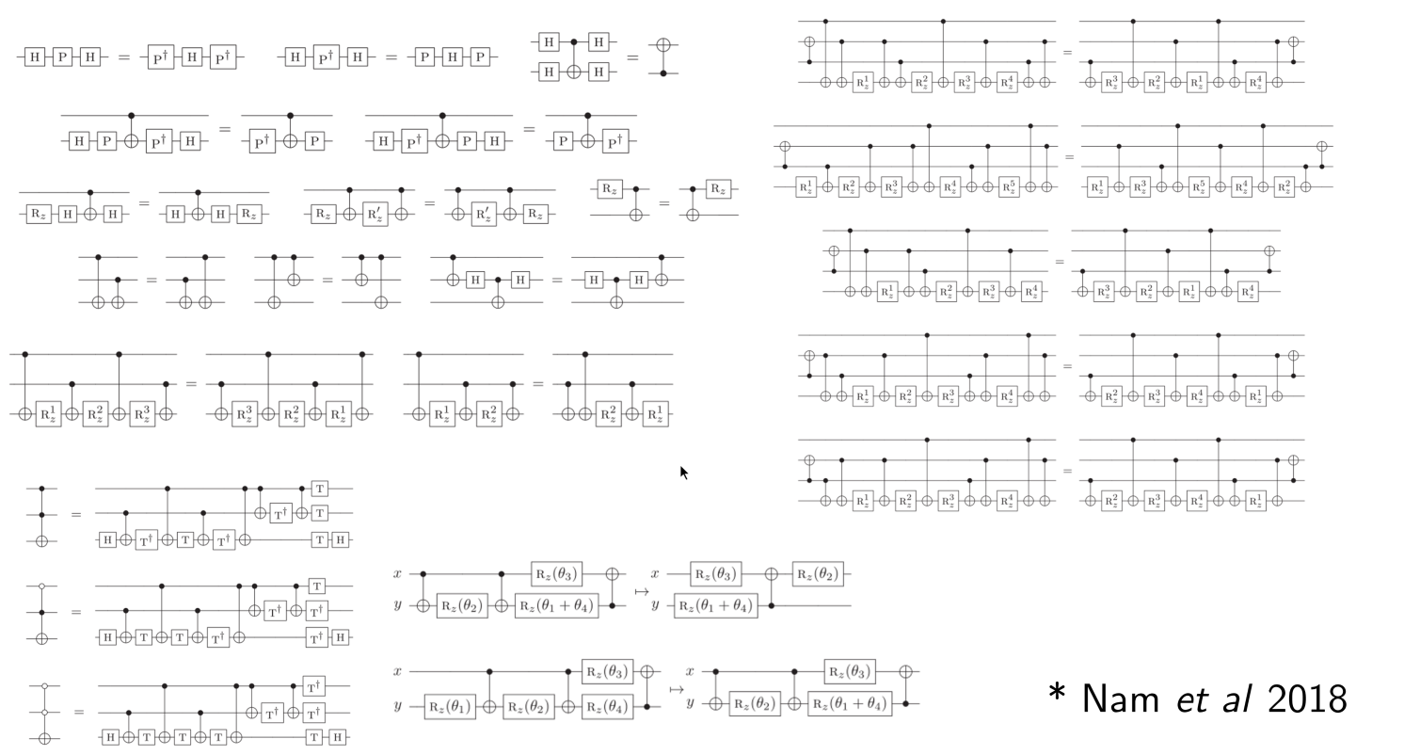
\includegraphics[width=\linewidth]{images/rewrite_rules_classical.png}
    \caption{Small subset of rewrite rules for classical circuit optimization
            {\cite{alexkissinger2020introductionzx}}}
    \label{fig:rewrite_rules_classical}
\end{figure}


\subsection{Quantum Circuit Optimization using the ZX-Calculus}

A more efficient approach for quantum circuit optimization is to use the ZX-Calculus. The ZX-Calculus is a graphical language for quantum computing, differing from the logic-gate representation by using connected nodes to represent operations on qubits. Since this new representation utilizes way fewer \textit{gate-types} than the classical representation, there exist way fewer rewrite rules.